% Tento soubor nahraďte vlastním souborem s obsahem práce.
%=========================================================================
% Autoři: Michal Bidlo, Bohuslav Křena, Jaroslav Dytrych, Petr Veigend a Adam Herout 2019
\chapter{Úvod}

Cieľom tejto bakalárskej práce je návrh architektúry a následná implementácia aplikácie určenej na extrakciu dát z webových stránok. V dnešnej dobe je pojem extrakcia dát používaný stále častejšie v spojitosti práve s webovými technológiami a webom samotným práve preto, že sa internet ako taký, a hlavne jeho obsah v podobe webových stránok, neustále rozširuje. Objem dát ktoré sa na webe nachádza sa zväčšuje neúprosnou rýchlosťou, a preto je zber údajov z rôznych webstránok stále zložitejší, a to nielen čo sa zložitosti štruktúry webu týka, ale vzhľadom na veľký počet webov sa zvyšuje aj časová náročnosť analýzy a následnej extrakcie dát.

Práve pre spomínanú expanziu internetu sa tejto téme venuje čoraz viac spoločností so snahou uľahčiť prístup k web scrapingu pre každodenných užívateľov, ale aj rôznych korporácií ktoré by o extrakciu dát z webových stránok mohli mať záujem. Pre neustáli vývoj webu je avšak nutné vyvíjať aj aplikácie, ktoré sú na extrakciu určené. 

Pri rozlišovaní takýchto aplikácií sa berie na vedomie hlavne požadovaný vstupný formát a jeho zložitosť, požadovaný výstupný formát a jeho využiteľnosť v praxi, a v neposlednom rade rýchlosť aplikácie z pohľadu extrakcie dát. 

Táto práca je zameraná hlavne na časť týkajúcu sa požadovaného vstupu aplikácie, kde je za cieľ požadovaný jednotný vstup vo forme Json súboru pozostávajúci z adries webových stránok, dátových typov, rozloženia objektov na webstránke, a požadované názvy extrahovaných informácií. Aplikácia sa následne pozerá na každú stránku zvlášť a určí výsledné údaje na základe poskytnutých relevantných informácií o štruktúre. Týmto spôsobom je možné definovať jeden vstup raz, a použiť ho na viaceré webové dokumenty bez nutnosti ďalšieho zásahu.

Prvá časť práce sa v kapitole \ref{aktualny_pristup} zaoberá aktuálnym prístupom k problematike, ako sa web scraping využíva v súčastnosti, aké sú štandardy a dostupné technológie, a porovnanie týchto prístupov z hľadiska využiteľnosti.

V druhej časti tejto práce sú v kapitole 3 popísané technológie ktoré je treba brať v úvahu pri návrhu, tvorbe a analýze aplikácie určenej na extrakciu dát. Jedná sa hlavne o technológie ktoré sa stali základným kameňom navrhnutej aplikácie, a o technológie na ktorých aplikácia stavia.

Kapitola 4 sa zameriava na analýzu a návrh architektúry aplikácie. Je založená na analýze špecifikácie a požiadavkov aplikácie, a popisuje postup návrhu aplikácie.

V 5. kapitole sú popísané jednotlivé detaily implementácie riešenia, a hlavná logika aplikácie.

6. kapitola sa následne venuje testovaní aplikácie za pomoci niekoľkých datasetov, a následnej analýze a vyhodnotení výsledkov ktoré aplikácia dosiahla.


\chapter{Aktuálny prístup k problematike Web Scrapingu}
\label{aktualny_pristup}

V tejto kapitole sú uvedené a popísané aktuálne prístupy ktoré sa používajú na extrakciu dát z webových dokumentov. Takáto extrakcia môže prebiehať online alebo offline, v závislosti na tom aké dáta a za akým cieľom chceme extrahovať.

Web scrapingu ako takému sa v súčastnosti venuje stále viac a viac spoločností, a preto nieje prekvapením že sa rozširujú nielen možnosti web scrapingových aplikácií, ale aj prístup takýchto aplikácií k priamej extrakcii dát.

Zároveň sa rozširuje pole pôsobnosti, a možnosti využitia takto extrahovaných dát. Preto je táto kapitola určená hlavne rozboru týchto metód. Poznatky získané z tohto rozboru zároveň pomôžu určiť smer ktorým sa návrh a vývoj aplikácie môžu uberať. 

\section{Web scraping}

Web scraping je jednou z foriem získavania údajov z webových stránok. Takéto získavanie údajov je možné buď priamo - World Wide Web za pomoci Hypertext Transfer Protokolu, alebo pomocou webového prehliadača (napr. Google Chrome). Za web scraping sa dá považovať aj manuálny zber dát za využitia ľudskej sily, ale všeobecne sa tým myslí využitie dedikovaného počítača ktorý túto prácu automatizuje. Tu sa môže jednať napríklad o jednoduché kopírovanie dát, alebo zložitejšie generovanie výstupných štruktúr napríklad vo formáte JSON. \cite{wiki:Web_scraping}

Automatizované získavanie informácií z webu sa dostalo do vývoja krátko po zavedení World Wide Web. Kvôli neustálemu vývoju technológií je však vo vývoji doteraz, a jeho možnosti sa neustále rozširujú. Prvé formy automatizovaných web scraperov boli určené primárne pre tvorbu databázy vyhľadávacieho indexu pre vývoj World Wide Web Vyhľadávače. Za jeden z prvých takýchto scraperov je preto považovaný World Wide Web Wanderer, ktorý bol vyvinutý v roku 1993 za účelom zmerania veľkosti celého internetu, a neskôr na indexáciu celého internetu. \cite{wiki:Web_scraping}

\section{Súčasné postupy}

Existujú rôzne prístupy k danej problematike, kde rozdiely sú jednoznačné hlavne pri spôsobe a type analýzy a extrakcie finálnych dát. Hlavným cieľom pri tvorbe aplikácie na takúto extrakciu dát je užívateľská prívetivosť, a jednoduchosť definovania vstupných požiadavkov. Postup ktorý aplikácie na extrakciu dát využívajú je prevažne rovnaký, a skladá sa z troch primárnych krokov:
\begin{enumerate}
  \item{Odoslanie GET požiadavku na webový server a následné obdržanie odpovedi}
  \item{Analýza extrahovaného HTML kódu na základe stromovej štruktúry}
  \item{Použitie zvoleného postupu na extrakciu dát a spracovanie hľadaného obsahu}
\end{enumerate}

Tieto kroky sú potom pri každej aplikácií mierne prispôsobené určeniu a typu implementácie. \cite{online:how_does_scraping_work}

\begin{figure}[hbt]
	\centering
	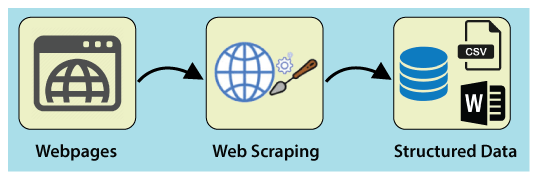
\includegraphics[width=0.5\textwidth]{obrazky-figures/web-scraping-using-python.png}
	\caption{Všeobecný postup ktorým sa aplikácia typu web scraper riadi. Prevzaté z Javatpoint \cite{WebScrap}}
	\label{WebScrap_img}
\end{figure}

\bigskip

Medzi najpopulárnejšie web scrapery patria aplikácie s jednoduchou point-and-click politikou, kde používateľ po inštalácií takejto aplikácie jednoducho zvolí webové dokumenty z ktorých chce extrakciu prevádzať, a následne interaktívne vyznačí dáta ktoré ho zaujímajú. Pre užívateľov ktorý nemajú príliš veľké skúsenosti s informačnými technológiami a nechcú platiť za túto službu nemalé peniaze rôznym korporáciám je to skrátka jediná možnosť.

\bigskip

Spomínaný prístup má samozrejme svoje výhody, medzi ktoré sa radí najmä spomínaná užívateľská prívetivosť a relatívne nízka cena, avšak v prípade potreby automatizácie takejto činnosti existujú na trhu lepšie riešenia. V prípade že je potrebná vysoká automatizácia, alebo sa jedná o veľké množstvo dát a stránok ktoré sú na extrakciu určené, je výhodnejšie použiť aplikáciu ktorá je ladená skôr na tento spôsob. Pri firmách ktoré sa venujú extrahovaniu údajov z webových stránok na profesionálnej úrovni sa počet prenesených dát v súčasnosti pohybuje už v petabajtoch, a počet extrahovaných webových stránok sa pohybuje v miliardách mesačne na jednu takúto firmu. 

Pri takto veľkých číslach narážajú spomínané firmy na rôzne problémy, ktoré rádový používateľ web scrapingovej aplikácie riešiť nemusí. Medzi takéto problémy sa radia v neposlednom rade napríklad:
\begin{itemize}
    \item {Náročnosť na hardvérový čas}
    \item {Limitovanie počtu možných GET dotazov}
    \item {Veľká diverzifikácia architektúry webových stránok}
    \item {Objem dát potrebný na prenesenie údajov a následné uloženie extrahovaných údajov}
\end{itemize}

Príklad ako sa takýmto problémom brániť alebo im priam predchádzať je v prípade limitovania počtu možných GET dotazov na jednu webovú stránku meniť IP adresy z ktorých sú GET dotazy odosielané. Ani to však nie vždy môže byť riešením, keďže stránky v dnešnej dobe môžu využívať rôzne ochrany proti web scrapingu, ako napríklad priamu detekciu človeka od robota alebo tzv. CAPTCHA\footnote{CAPTCHA - Completely Automated Public Turing test to tell Computers and Humans Apart.} .\cite{JanCurna:online} 

Web scraping má teda svoje výhody, ale aj nevýhody. Tieto sú popísané podrobnejšie v nasledujúcej časti tejto kapitoly.

\section{Výhody, nevýhody, a využitie web scrapingu}

Web scraping má v súčastnosti viac možností a oblastí využitia ako tomu bolo v minulosti. Toto je dané hlavne neustálim rozširovaním sa internetu ako celku. V počiatkoch internetu sa aplikácie typu web scraper nazývali skôr crawler, a využívali prevažne na indexáciu obsahu, a nie na zber, extrakciu a analýzu dát tak ako je tomu teraz. 

Web scraper je ale aplikácia ktorá je založená presne na tých fundamentálnych základoch ako spomínaný crawler, s jediným rozdielom a to tým, že jeho úlohou je zber dát. Takýto zber môže prebiehať napríklad kopírovaním dát do databázy. V mnohých prípadoch sú aplikácie typu scraper využívané veľkými korporáciami ako napríklad Microsoft, Amazon alebo Google na cielenie zobrazovaných reklám tak, aby boli pre užívateľa ako jednotlivca relevantné.\cite{online:how_does_scraping_work}

\bigskip

Jednotlivé prípady využitia takejto aplikácie sa neustále rozširujú, obecne ale platí že jeho využitie spadá do nasledovných kategórií:

\begin{itemize}
    \item {Monitorovanie ceny produktov}
    \item {Získavanie údajov o nových produktoch na trhu}
    \item {Analýza konkurencie}
    \item {Evidovanie údajov o konkrétnej doméne podľa druhu záujmu}
    \item {Monitorovanie ceny leteniek}
\end{itemize}

A mnohé ďalšie prípady. Údaje extrahované touto metódou môžu byť následne využité na širšie pochopenie vývoja udalostí napríklad na trhu, alebo u konkurencie.

Web scraping má teda jasné výhody čo sa kolekcie dát týka. Patria medzi ne už spomínané monitorovanie konkurencie, cien produktov a analýza rôznych dát. V neposlednom rade ale treba zmieniť aj výhody z pohľadu technológie samotnej. Medzi ne patria napríklad:

\begin{itemize}
    \item {Rýchlo sa rozvíjajúce technológie}
    \item {Automatizovanie monotónnych činností}
    \item {Zber obsiahleho množstva dát, ktorý by bol manuálne nemožný}
    \item {V porovnaní s manuálnym zberom dát exponenciálne rýchlejšie výsledky}
\end{itemize}

Každá technológia a jej využitie má však aj svoje nevýhody. V porovnaní s manuálnym zberom dát, ktoré môže byť rozumné ak sa jedná o ojedinelú prípadne unikátnu udalosť, kedy je takýto zber potrebné vykonať jeden krát za dlhé obdobie, sa tvorba alebo priame využitie web scrapera očakáva až v prípade že sa daná akcia musí vykonávať automatizovane a v určitých časových intervaloch. \cite{WebScrap}

V takom prípade je potreba zvážiť aj rôzne prvky pri nielen prevádzke, ale aj samotnom vytváraní a následnom používaní web scrapera. Medzi najhlavnejšie nevýhody sa preto radí najmä:

\begin{itemize}
    \item {Znalosť kódovania a programovania}
    \item {IP Detekcia a CAPTCHA}
    \item {Ku každej stránke je potreba pristupovať individuálne}
\end{itemize}

Zároveň treba spomenúť fakt, že dynamické stránky môžu meniť svoju štruktúru, a preto nemôžme zabúdať na údržbu web scrapera nielen z pohľadu úrovne bezpečnosti programu, ale aj z pohľadu údajov ktoré web scraper prijíma. V prípade že webová stránka zmení štruktúru tak, že aktuálna konfigurácia web scrapera nedokáže pokračovať v extrahovaní údajov tak ako predtým, je potrebné v mnohých prípadoch stránku znova analyzovať, a v prípade že je web scraper neschopný efektívne využiť algoritmy ktoré v minulosti fungovali, v niektorých prípadoch aj dodatočne zanalyzovať prístupy web scrapera a upraviť jeho logiku tak, aby mohol v extrahovaní pokračovať.

\section{Metódy využívané v súčastnosti}

V prípade že nás zaujíma len priama extrakcia dát, v dnešnej dobe je na výber z mnohých aplikácií ktoré sú pripravené na použitie, a tak nieje treba programovať aplikácie znova. Každá má však svoje vlastné postupy pri extrakcii, a z toho plynie fakt že nie každá takáto aplikácia dokáže splniť požadované zadanie. Medzi najznámejšie aplikácie v tomto odvetví však patria hlavne:

\begin{itemize}
    \item {Scrapping-bot}
    \item {Octoparse}
    \item {Import.io}
    \item {Dexi.io}
    \item {Outwit}
\end{itemize}

V niektorých prípadoch nám stačí jednoduché rozšírenie do prehliadača (napr. Google Chrome) ktoré sú efektívne hlavne pri menšom počte webstránok určených na scraping. \cite{WebScrap}

\bigskip

Pokiaľ však chceme vytvoriť vlastný program alebo aplikáciu typu web scraper, je potrebné rozlišovať na úrovni technológií dostupných pri programovaní. V prvom rade je treba vziať do úvahy programovací jazyk. V takom prípade je na výber rovno z niekoľko volne dostupných programovacích jazykov. Medzi dva najpopulárnejšie však patria hlavne Python, a Node.js. Každý má však znova svoje výhody a nevýhody, a preto je treba zvážiť na aké účely bude web scraper používaný. Vo všeobecnosti je populárnejší práve prvý spomínaný Python, vďaka jeho popularite z pohľadu jednoduchosti písania čistého kódu, komunity, a podpory ktorá je mu venovaná. Python ponúka veľké množstvo frameworkov, z ktorých tie najpopulárnejšie zahŕňajú hlavne Selenium a Scrapy, ktoré som samozrejme zohľadnil pri výbere vhodného frameworku na vytvorenie web scrapera.

Na druhej strane Node.js stavia na základoch Javascriptu, ktorý je vyvíjaný priamo pre prácu s web stránkami. Kým Python je lepší čo sa týka podpory a rozšírenosti frameworkov, Javascript má výhodu v lepšej integrácií nielen s webovými stránkami ako takými, ale aj s webovými prehliadačmi samotnými. Python v mnohých prípadoch vyžaduje driver na komunikáciu s prehliadačom, a podpora dynamických stránok je znova jednoznačne lepšia pomocou Javascriptu, práve kvôli jeho spomínanej lepšej integrácií a faktom, že Javascript je jednou z hlavných súčastí dynamických moderných webových stránok. Javascript je jednou z hlavných súčastí modernej webovej stránky, ktorá sa skladá ešte z HTML a CSS. Jeho úlohou je hlavne vytváranie dynamického obsahu vytvárajúceho dojem že webová stránka s užívateľom interaguje. Vo väčšine prípadov beží iba na strane klienta, takže dynamickosť samotná nezaťažuje server. Zároveň je v mnohých prípadoch využívaná asynchrónnosť\footnote{Asynchrónnosť znamená v tomto prípade neblokovanie prehliadačových prostriedkov a načítavanie obsahu za behu webstránky.} tohto programovacieho jazyka, na zlepšenie odozvy a interakcie. Práve tento fakt sa stáva rozdielovým faktorom pri extrakcii dát z webových stránok, keďže obsah webovej stránky sa v mnohých prípadoch môže načítavať asynchrónne a nezávisle od ostatných častí webu. Z môjho vlastného rozboru a výskumu som zistil, že dynamickosť a asynchrónnosť stránok je prvok ktorý je lepšie zvládaný za pomoci Javascriptu. \cite{The5Best}\cite{Javascript}

\bigskip

Rozhodnutie používať Javascript som učinil zároveň s predpokladom využitia jedného z jeho volne dostupných frameworkov, a zároveň som zohľadnil svoje predošlé skúsenosti práve so spomínaným jazykom. K tomuto rozhodnutiu prispel aj fakt, že v dnešnej dobe je dynamika stránok takmer štandard, a tu hrá úloha Javascriptu veľkú rolu. V procese výberu frameworku som zohľadňoval hlavne integráciu daného frameworku s prehliadačom, výbornú podporu dynamických stránok a asynchrónnosť ktorá je pri takejto aplikácii kľúčová.

Ako prvý framewrok spomeniem určite Apify SDK, za ktorým stojí Česká firma Apify Technologies\footnote{{\url{https://apify.com/}}}.\cite{JanCurna:online} Práve Apify ma totiž inšpirovalo v rôznych odvetviach vývoja. Medzi najznámejšie technológie ktoré používajú Javascript patria najmä:

\begin{itemize}
    \item {Apify SDK}
    \item {Puppeteer}
    \item {Cheerio}
\end{itemize}

Z pomedzi týchto technológií ktoré zdieľajú niektoré základné funkcie bola na zostavenie výslednej aplikácie použitá technológia Puppeteer. Puppeteer je zároveň jedna z technológií využívaných práve spomínanou Českou firmou Apify. 

V porovnaní s technológiou Cheerio má Puppeteer svoje výhody. V niektorých faktoroch vyhráva ale aj Cheerio, a preto je treba zvážiť hlavne nasledovné:

\begin{itemize}
    \item {Možnosť scrapingu dynamických stránok}
    \item {Funkcionality a možnosti}
    \item {Kompatibilnosť webových technológií}
    \item {Rýchlosť analýzy a extrakcie}
\end{itemize}

V prvom rade treba zvážiť aktuálnu situáciu a technológie ktoré sa na webe vyskytujú. 95\% webových stránok v súčastnosti používa Javascript, takže predpoklad že moderné weby budú obsahovať dynamický obsah je prevažne jasný, a preto treba s takýmto obsahom počítať. Node.js ktorý je postavený na Javascripte je zároveň najrýchlejšie sa rozširujúcou technológiou ktorú web využíva. V čase písania má Node.js viac ako 1.5 milióna dostupných rozširujúcich balíčkov, a jeho náskok je v súčasnej dobe jednoznačný.\cite{HowPopular} 

\begin{figure}[hbt]
	\centering
	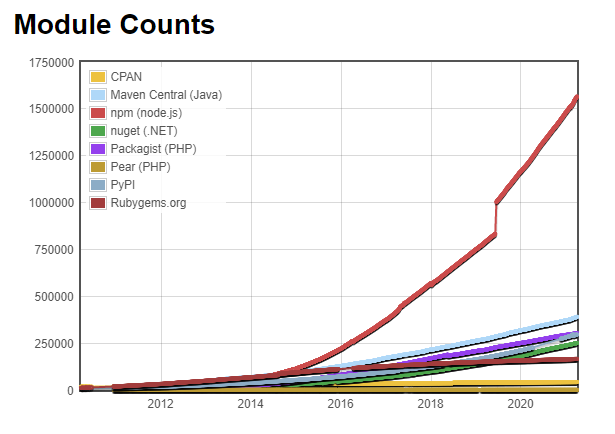
\includegraphics[width=0.5\textwidth]{obrazky-figures/modules.png}
	\caption{Porovnanie najpopulárnejších technológií a vývoj počtu ich modulov. Zdroj \cite{Moduleco}}
	\label{Moduleco_img}
\end{figure}

\bigskip

Pri porovnávaní technológií Puppeteer a Cheerio je na prvý pohľad jednoznačné čo majú spoločné, a v čom naopak každá z nich vyniká. Tieto poznatky pomôžu jednoznačne určiť technológiu na základe požiadavkov ktoré vznikli zároveň s výberom témy tejto práce.

Cheerio a Puppeteer sú technológie založené na Node.js, a patria medzi najpopulárnejšie technológie v tomto odvetví. Ich jednoznačné vlastnosti však definujú nielen ich možné prípady použitia, ale zároveň schopnosti a rýchlosť akou sú schopné dosiahnuť očakávané výsledky. 

Puppeteer je technológia ktorá je vyvíjaná za účelom automatizácie webového prehliadača, zatiaľčo hlavným určením Cheeria je web scraping samotný. Tým že je Cheerio určené priamo na požadovanú úlohu je v tomto ohľade rýchlejšie a výhodnejšie čo sa nášho požiadavku týka. Cheerio je zároveň multiplatformné, a dokáže pracovať ako s prehliadačom Firefox, tak s prehliadačom Google Chrome. Na druhú stranu Puppeteer je viazaný iba na prehliadač Google Chrome vo forme Chromium. Puppeteer má priamo kontrolu nad prehliadačom, takže je možné ovládať prehliadač ako celok. Tento fakt sa dá brať aj ako výhoda aj ako nevýhoda, keďže je to pravdepodobne jeden z dôvodov prečo je Puppeteer pomalší vo vykonávaní funkcie Web Scrapera. Puppeteer však prináša schopnosť plynulej práce s Javascriptom na webovej stránke, dokáže parsovať aj webové stránky postavené na moderných technológiách ako React alebo Angular, ktoré sú v dnešnej dobe na vzostupe pre ich moderné prvky. Z priamej integrácie s prehliadačom vyplýva aj fakt že Puppeteer dokáže vytvárať snímky obrazovky počas načítavania a pracovania s webovou stránkou. Zároveň podporuje technológiu XML, a nerobí mu problém ako čítanie, tak ani parsovanie a priame spúšťanie Javascriptových funkcií. \cite{Differences}

Práve podpora dodatočných funkcií a možnosť parsovania dynamických stránok s Javascriptom ma presvedčili o rozširovaní poznatkov technológie Puppeteer, a jej následné využitie pri návrhu architektúry a implementácie výslednej aplikácie.

\chapter{Technológie}
